\documentclass[a4paper,12pt]{article}


%%% Работа с русским языком
\usepackage{cmap}					% поиск в PDF
\usepackage{mathtext} 				% русские буквы в формулах
\usepackage[T2A]{fontenc}			% кодировка
\usepackage[utf8]{inputenc}			% кодировка исходного текста
\usepackage[english,russian]{babel}	% локализация и переносы
\usepackage{indentfirst}
\frenchspacing

\newcommand{\vyp}{\ensuremath{\hookrightarrow}}
\renewcommand{\epsilon}{\ensuremath{\varepsilon}}
\renewcommand{\phi}{\ensuremath{\varphi}}
\renewcommand{\kappa}{\ensuremath{\varkappa}}
\renewcommand{\le}{\ensuremath{\leqslant}}
\renewcommand{\leq}{\ensuremath{\leqslant}}
\renewcommand{\ge}{\ensuremath{\geqslant}}
\renewcommand{\geq}{\ensuremath{\geqslant}}
\renewcommand{\emptyset}{\varnothing}
\newcommand{\Ra}{\ensuremath{\Rightarrow}}
\newcommand{\ra}{\ensuremath{\rightarrow}}
\newcommand{\LRa}{\ensuremath{\Leftrightarrow}}
\newcommand{\tbf}{\textbf}
\newcommand{\ov}{\ensuremath{\overline}}
\newcommand{\CC}{\ensuremath{\mathbb{C}}}
\newcommand{\RR}{\ensuremath{\mathbb{R}}}
\newcommand{\NN}{\ensuremath{\mathbb{N}}}
\newcommand{\QQ}{\ensuremath{\mathbb{Q}}}
\newcommand{\ZZ}{\ensuremath{\mathbb{Z}}}

%%% Дополнительная работа с математикой
\usepackage{amsmath,amsfonts,amssymb,amsthm,mathtools} % AMS
\usepackage{icomma} % "Умная" запятая: $0,2$ --- число, $0, 2$ --- перечисление

%% Номера формул
%\mathtoolsset{showonlyrefs=true} % Показывать номера только у тех формул, на которые есть \eqref{} в тексте.
%\usepackage{leqno} % Нумереация формул слева

%% Свои команды
\DeclareMathOperator{\sgn}{\mathop{sgn}}

%% Перенос знаков в формулах (по Львовскому)
\newcommand*{\hm}[1]{#1\nobreak\discretionary{}
{\hbox{$\mathsurround=0pt #1$}}{}}



%%% Работа с картинками
\usepackage{graphicx}  % Для вставки рисунков
\graphicspath{{images/}{images2/}}  % папки с картинками
\setlength\fboxsep{3pt} % Отступ рамки \fbox{} от рисунка
\setlength\fboxrule{1pt} % Толщина линий рамки \fbox{}
\usepackage{wrapfig} % Обтекание рисунков текстом

%%% Работа с таблицами
\usepackage{array,tabularx,tabulary,booktabs} % Дополнительная работа с таблицами
\usepackage{longtable}  % Длинные таблицы
\usepackage{multirow} % Слияние строк в таблице

%%% Теоремы
\theoremstyle{plain} % Это стиль по умолчанию, его можно не переопределять.
\newtheorem{theorem}{Теорема}[section]
\newtheorem{proposition}[theorem]{Утверждение}
 
\theoremstyle{definition} % "Определение"
\newtheorem{corollary}{Следствие}[theorem]
\newtheorem{problem}{Задача}[section]
 
\theoremstyle{remark} % "Примечание"
\newtheorem*{nonum}{Решение}

%%% Программирование
\usepackage{etoolbox} % логические операторы

%%% Страница
\usepackage{extsizes} % Возможность сделать 14-й шрифт
\usepackage{geometry} % Простой способ задавать поля
	\geometry{top=20mm}
	\geometry{bottom=20mm}
	\geometry{left=5mm}
	\geometry{right=15mm}
 %
\usepackage{fancyhdr} % Колонтитулы
 	\pagestyle{fancy}
 	\renewcommand{\headrulewidth}{1pt}  % Толщина линейки, отчеркивающей верхний колонтитул
%\fancypagestyle{firstpage}{
	\rhead{\large{Исыпов Илья}}
%}
% 	\lfoot{Нижний левый}
% 	\rfoot{\large{Рябых Владислав, Б05-905}}
% 	\rhead{Верхний правый]}
% 	\chead{Верхний в центре}
 	\lhead{\large{Рябых Владислав}}
%	\cfoot{Нижний в центре} % По умолчанию здесь номер страницы

\usepackage{setspace} % Интерлиньяж
\onehalfspacing % Интерлиньяж 1.5
%\doublespacing % Интерлиньяж 2
%\singlespacing % Интерлиньяж 1

\usepackage{lastpage} % Узнать, сколько всего страниц в документе.

\usepackage{soul} % Модификаторы начертания

\usepackage{hyperref}
\usepackage[usenames,dvipsnames,svgnames,table,rgb]{xcolor}
\hypersetup{				% Гиперссылки
    unicode=true,           % русские буквы в раздела PDF
    pdftitle={Заголовок},   % Заголовок
    pdfauthor={Автор},      % Автор
    pdfsubject={Тема},      % Тема
    pdfcreator={Создатель}, % Создатель
    pdfproducer={Производитель}, % Производитель
    pdfkeywords={keyword1} {key2} {key3}, % Ключевые слова
    colorlinks=true,       	% false: ссылки в рамках; true: цветные ссылки
    linkcolor=red,          % внутренние ссылки
    citecolor=black,        % на библиографию
    filecolor=magenta,      % на файлы
    urlcolor=cyan           % на URL
}

\usepackage{csquotes} % Еще инструменты для ссылок

%\usepackage[style=authoryear,maxcitenames=2,backend=biber,sorting=nty]{biblatex}

\usepackage{multicol} % Несколько колонок

\usepackage{tikz} % Работа с графикой
\usepackage{pgfplots}
\usepackage{pgfplotstable}

\usepackage{caption}
\long\def\comment{}
\setlength{\abovecaptionskip}{7pt}
\setlength{\belowcaptionskip}{7pt}
\usepackage{enumitem}
\mathtoolsset{showonlyrefs}

\begin{document}

\begin{titlepage}
	\begin{center}
		
		\textsc{\LARGE Московский\\[-0.2cm]Физико-Технический Институт\\[0.1cm]\large (национальный исследовательский университет)}\\[1.5cm] 
		
	
\includegraphics[width=0.3\textwidth]{hv_s_no_bg.png}~\\[1cm]

	\textsc{\Large Оптика. \\ Лабораторный практикум. }\\[0.2cm]

	% Title
	\HRule \\[0.4cm]
	{ \LARGE \bfseries Лабораторная работа № 4.7.3 \\ Поляризация. \\[0.4cm] }

	\HRule \\[1.5cm]
		
		% Author and supervisor
		\noindent
		\begin{minipage}{0.4\textwidth}
			\begin{flushleft} \large
			\end{flushleft}
		\end{minipage}%
		\begin{minipage}{0.4\textwidth}
			\begin{flushright} \large
			\end{flushright}
		\end{minipage}
		
		
		\large{\begin{flushright}
				\vfill
				\textbf{Выполнил}:\\
				\textbf{Рябых Владислав,\\}
%				\textbf{Исыпов Илья\\}
				\textbf{группа Б05-905}
		\end{flushright}}
		
		
		{\large \today}\\
		
		
	\end{center}
\end{titlepage}

\subsubsection*{Цель работы:} ознакомление с методами получения и анализа поляризованного света.

\subsubsection*{Оборудование:} оптическая скамья с осветителем; зелёный светофильтр; два поляроида; чёрное зеркало; полированная эбонитовая пластинка; стопа стеклянных пластинок; слюдяные пластинки разной толщины; пластинки в 1/4 и 1/2 длины волны; пластинка в одну длину волны для зелёного света (пластинка чувствительного оттенка).

\section*{Теория}

\subsection*{Определение направления разрешённой плоскости колебаний поляроида}

Определить направление разрешённых колебаний поляроида проще всего с помощью чёрного зеркала.

При падении света на отражающую поверхность под углом Брюстера, свет в отражённом луче почти полностью поляризован, а вектор E
параллелен отражающей поверхности ("<правило иголки">). Луч света,
прошедший поляроид и отразившийся от чёрного зеркала, имеет минимальную интенсивность при выполнении двух условий: во-первых, свет
падает на отражающую поверхность под углом Брюстера и, во-вторых,
в падающем пучке вектор E лежит в плоскости падения.

Вращая поляроид вокруг направления луча и чёрное зеркало вокруг
оси, перпендикулярной лучу, методом последовательных приближений
можно добиться минимальной яркости луча, отражённого от зеркала,
и таким образом определить разрешённое направление поляроида.

Измеряя угол поворота зеркала (угол Брюстера), нетрудно определить коэффициент преломления материала, из которого изготовлено
зеркало. Описанный метод часто используется для измерения коэффициента преломления непрозрачных диэлектриков.

\subsection*{Получение эллиптически поляризованного света}

Эллиптически поляризованный свет можно получить из линейно поляризованного с
помощью двоякопреломляющих кристаллических пластинок.

Двоякопреломляющая пластинка имеет два взаимно перпендикулярных главных направления, совпадающих с осями эллипсоида диэлектрической проницаемости. Волны, поляризованные вдоль главных направлений, распространяются в пластинке с разными скоростями, не изменяя характера своей поляризации. Эти волны называются главными. Мы будем обозначать показатели преломления для главных волн через $ n_x $ и $ n_y $, где $ x $ и $ y $ --- главные направления кристаллической пластинки (рис. \ref{ris 1}).

\begin{figure}[h] 
	\centering
	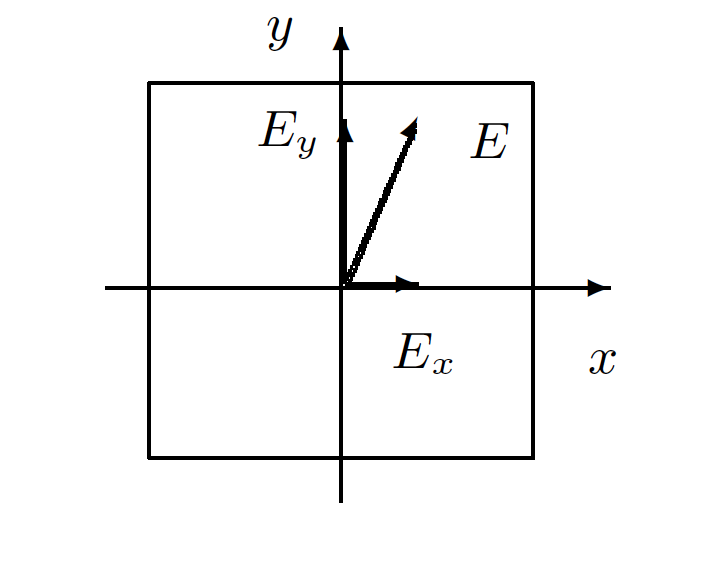
\includegraphics[width=0.3\linewidth]{1}
	\caption{Разложение линейно поляризованного света по главным направлениям двоякопреломляющей пластинки}
	\label{ris 1}
\end{figure}

Пусть на пластинку падает линейно поляризованная волна, электрический вектор которой ориентирован под некоторым углом $ \alpha $ к оси
$ x $. Разложим вектор $ \vec{E} $ на составляющие $ E_x $ и $ E_y $. На входе пластинки $ E_x $ и $ E_y $ находятся в фазе. На выходе из-за разности скоростей между ними появляется разность хода $ d(n_x - n_y) $, при этом сдвиг фаз определяется соотношением

\begin{equation}\label{}
	\Delta \phi =  \dfrac{2\pi}{m} = k d(n_x - n_y)
\end{equation}
Как уже отмечалось, при сложении двух взаимно перпендикулярных колебаний, обладающих некоторым сдвигом фаз, образуется колебание, поляризованное по эллипсу.

Рассмотрим практически важные частные случаи.

\begin{enumerate}[label=\alph*)]
	
	\item Пластинка даёт сдвиг фаз $ 2\pi $ (пластинка в длину волны $ \lambda $). В результате сложения волн на выходе пластинки образуется линейно поляризованная волна с тем же направлением колебаний, что и в падающей волне.
	
	\item Пластинка даёт сдвиг фаз $ \pi $ (пластинка в полдлины волны $ \lambda / 2 $). На выходе пластинки снова образуется линейно поляризованная волна. Направление $ bb' $ колебаний этой волны повёрнуто относительно направления $ aa' $ колебаний падающей волны (рис. \ref{ris 2}). Как нетрудно сообразить, направление $ bb' $ является зеркальным отображением направления $ aa' $ относительно одного из главных направлений пластинки. Такую пластинку используют для поворота направления колебаний линейно поляризованного света.
	
	\item Пластинка создаёт между колебаниями сдвиг фаз $ \pi/2 $ (пластинка
	в четверть длины волны). При сложении двух взаимно перпендикулярных колебаний, имеющих разность фаз $ \pi/2 $, образуется эллипс, главные оси которого совпадают с координатными осями $ x $ и $ y $. При равенстве амплитуд возникает круговая поляризация.
	
\end{enumerate}

\begin{figure}[h] 
	\centering
	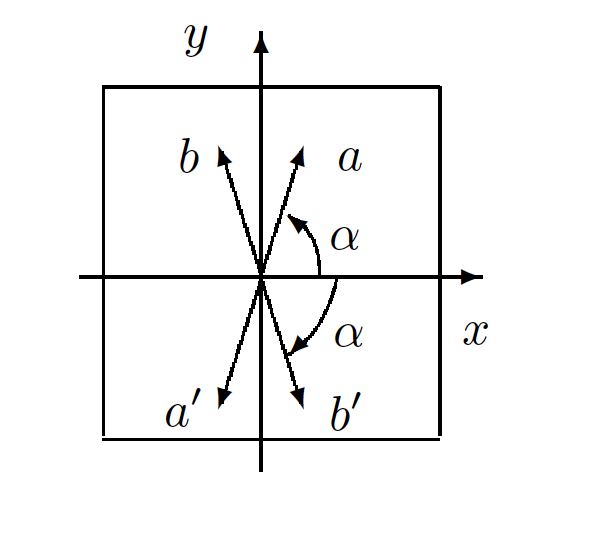
\includegraphics[width=0.3\linewidth]{2}
	\caption{Поворот направления колебаний с помощью пластинки в $ \lambda / 2 $}
	\label{ris 2}
\end{figure}

Следует отметить, что, говоря о пластинках $ \lambda , \lambda/2, \lambda/4  $ и т. д., всегда подразумевают какую-либо вполне определённую монохроматическую
компоненту (например, пластинка $ \lambda/2 $ для зелёного света). Если на двоякопреломляющую пластинку падает не монохроматический свет, то на
выходе из неё для разных спектральных компонент эллипсы поляризации будут различными.

\subsection*{Анализ эллиптически поляризованного света}

Анализ эллиптически поляризованного света сводится к нахождению главных осей
эллипса поляризации и к определению направления вращения электрического вектора.

Главные оси эллипса поляризации определяются с помощью анализатора по максимуму и минимуму интенсивности проходящего света.
Направление вращения электрического вектора может быть найдено с помощью пластинки в четверть длины волны, для которой известно, какая из главных волн, $ E_x $ или $ E_y $, имеет б\'{o}льшую скорость распространения (и соответственно меньшее значение показателя преломления).

Выберем для определённости координатные оси $x$ и $y$ на пластинке
так, чтобы $ n_x < n_y $. В этом случае главная волна $ E_x $ имеет большую
скорость распространения. Поместим такую пластинку на пути эллиптически поляризованного света и совместим главные направления пластинки $ \lambda/4 $ с главными осями эллипса поляризации. На выходе из этой пластинки сдвиг фаз между $ E_x $ и $ E_y $ вместо $ \pi/2 $ станет равным нулю или $ \pi $. Свет окажется линейно поляризованным. Из двух возможных значений сдвига фаз, 0 или $ \pi $, реализуется одно: то, которое соответствует имеющемуся в волне направлению вращения электрического вектора.

Рассмотрим, например, случай, когда электрический вектор в эллиптически поляризованной волне вращается против часовой стрелки,
если смотреть навстречу лучу. В этом случае, очевидно, в волне, падающей на пластинку в $ \lambda/4 $, колебание $ E_y $ отстаёт по фазе на $ \pi/2 $ от
колебания $ E_x $. При прохождении через пластинку разность фаз увеличивается до $ \pi $. Таким образом на выходе из пластинки возникают линейно поляризованные волны со сдвигом фаз $ \pi $. Сложение этих волн даёт плоскополяризованную волну, электрический вектор которой располагается во втором и четвёртом квадрантах координатной системы
$ x, y $.

Рассуждая аналогичным образом, найдём, что при вращении электрического вектора по часовой стрелке направление колебаний в линейно поляризованной волне, выходящей из пластинки, располагается в первом и третьем квадрантах. Определяя направление колебаний на выходе из пластинки с помощью поляроида, можно, таким образом, определить характер эллиптической поляризации (вращение против или по часовой стрелке).

\subsection*{Пластинка чувствительного оттенка}

Выше предполагалось известным, какому из двух главных направлений пластинки в четверть длины волны соответствует большая скорость распространения света.
Установить это можно различными способами, например с помощью
пластинки чувствительного оттенка (так называют пластинку в $ \lambda $
для зелёной спектральной компоненты, $ \lambda = 560 $ нм).

Пластинка имеет форму стрелы (рис. \ref{ris 3}), вдоль оси которой расположено главное направление, соответствующее большей скорости распространения.

\begin{figure}[h] 
	\centering
	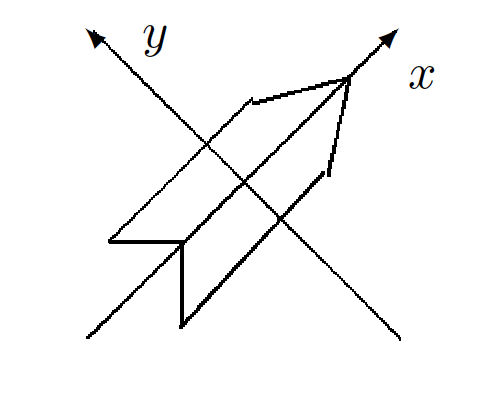
\includegraphics[width=0.3\linewidth]{3}
	\caption{Пластинка чувствительного оттенка}
	\label{ris 3}
\end{figure}

Если пластинка чувствительного оттенка помещена между скрещенными поляроидами и главные направления пластинки не параллельны направлениям разрешённых колебаний поляроидов, то при освещении белым светом пластинка кажется окрашенной в лилово-красный цвет.
Это объясняется тем, что зелёная компонента линейно поляризованного света при прохождении пластинки не меняет поляризации и задерживается вторым поляроидом. Для красной и фиолетовой компонент пластинка создаёт сдвиг фаз, несколько отличный от $ 2\pi $. На выходе
из пластинки красная и фиолетовая компоненты оказываются поэтому эллиптически поляризованными и частично проходят через второй поляроид. Таким образом, в известном смысле наблюдаемый в указанном опыте цвет пластинки дополнителен к зелёному.

Если между скрещенными поляроидами поместить пластинку чувствительного оттенка
($ \lambda $) и пластинку в $ \lambda/4 $ так, чтобы их главные направления совпадали, цвет пластинки изменится. Если у пластинки чувствительного оттенка и пластинки в $ \lambda/4  $ совпадут главные направления, соответствующие большей скорости распространения, то разность хода между $ E_x $ и $ E_y $ для зелёного света составит уже $ 5\lambda/4 $. Это соответствует разности хода в $ \lambda $ для света с большей длиной волны, т. е. для "<более красного"> света. При освещении этих пластинок (напомним, что они расположены между скрещенными поляроидами) белым светом теперь погасится не зелёная, а красная часть спектра, и проходящий свет будет казаться зеленовато-голубым. Если же главные направления, соответствующие большей скорости распространения, у пластинки чувствительного оттенка и у пластинки в $ \lambda/4 $ окажутся перпендикулярными, то проходящий свет приобретёт
оранжево-желтую окраску (погасится фиолетово-голубая часть спектра).

Изменение цвета позволяет, таким образом, определить, какое из
главных направлений пластинки в $ \lambda/4 $ соответствует большей скорости
распространения.

\subsection*{Интерференция поляризованных лучей}

Тонкие двоякопреломляющие пластинки, помещённые между поляроидами, кажутся окрашенными. Эта окраска может быть истолкована как результат интерференции поляризованных лучей. На рис. \ref{ris 4} представлена схема для случая скрещенных поляроидов.

\begin{figure}[h] 
	\centering
	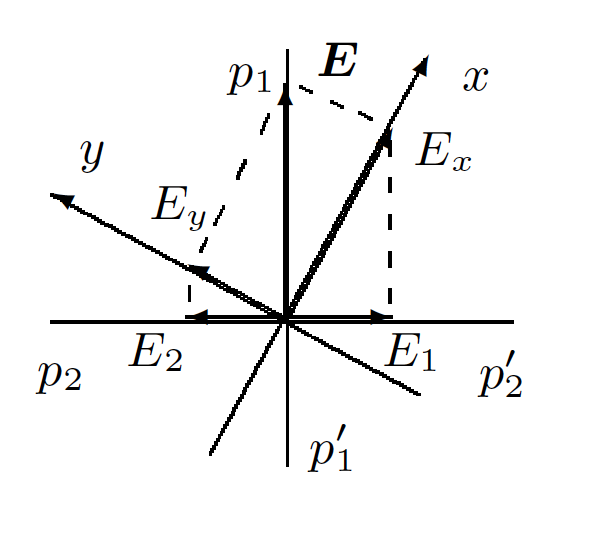
\includegraphics[width=0.3\linewidth]{4}
	\caption{К объяснению интерференции поляризованных лучей}
	\label{ris 4}
\end{figure}

Здесь $ p_1p_1' $ --- разрешённое направление колебаний поляризатора
(первого поляроида); $ x, y $~---~координатная система, связанная с главными направлениями двоякопреломляющей пластинки;

$ p_2p_2' $~---~разрешённое направление колебаний анализатора (второго поляроида). Волны $ E_x  $ и $ E_y $ на выходе из пластинки когерентны, но не могут интерферировать, так как $ E_x \perp  E_y $. Волны $ E_1 $ и $ E_2 $ на выходе второго поляроида также являются когерентными и к тому же поляризованы в одной плоскости. Эти волны интерферируют между собой. Результат интерференции определяется зависящим от длины волны сдвигом фаз между $ E_1 $ и $ E_2 $. В результате интерференции поляризованных лучей пластинка, освещаемая белым светом, кажется окрашенной.

Если поворачивать двоякопреломляющую пластинку, расположенную между
скрещенными поляроидами, то соотношение амплитуд волн $ E_1 $ и $ E_2 $ и разность фаз между ними не изменяются. Это означает, что цвет пластинки при её поворотах не меняется, а меняется только интенсивность света. За один оборот пластинки интенсивность четыре раза обращается в нуль~---~это происходит при совпадении главных направлений
$ x $ и $ y $ с разрешёнными направлениями колебаний поляроидов.

Если же двоякопреломляющую пластинку оставить неподвижной, а второй поляроид повернуть так, чтобы разрешённые направления $ p_1p_1' $ и $ p_2p_2' $ совпали, то волны $ E_1 $ и $ E_2 $ приобретают дополнительный фазовый сдвиг на $ \pi $ для всех спектральных компонент; при этом их амплитуды изменятся так, что цвет пластинки изменится на дополнительный. 

\clearpage

\section*{Ход работы}

\subsection*{Определение разрешенных направлений поляроида}

\begin{figure}[h] 
	\centering
	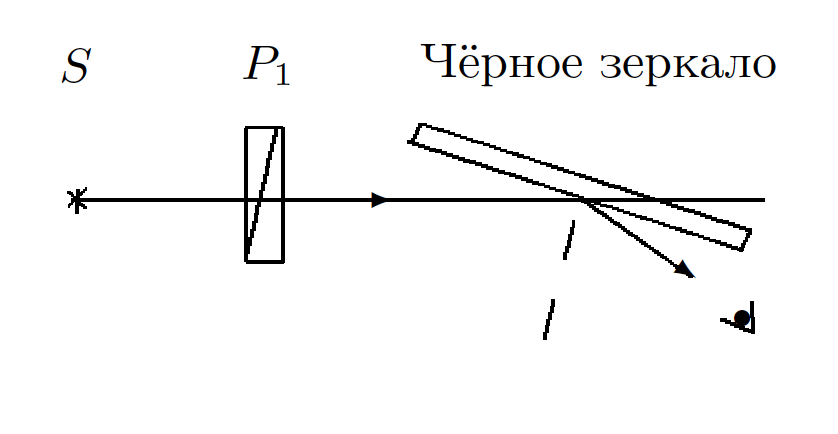
\includegraphics[width=0.3\linewidth]{5}
	\caption{Определение разрешенных направлений поляроида}
	\label{ris 5}
\end{figure}

Собираем оптическую схему, изображённую на рис. \ref{ris 5}. Будем поворачивать поляроид, находя минимальную яркость отражения при угле чёрного зеркала, равном $45^\circ$ 

Затем поворачиваем зеркало, опять же, добиваясь минимальной яркости отражения. Запишем показания на лимбе поляроида~---~они и будут задавать разрешённые направления поляроидов:

\[\phi_1 = 3^\circ \pm 1^\circ \ \ \ \ \ \ \ \ \phi_2 = 36^\circ \pm 1^\circ\]

\subsection*{Определение показателя преломления эбонита}

Поставим на скамью вместо чёрного зеркала (рис. \ref{ris 5}) эбонитовую
пластинку. Выставляя пластинку перпендикулярно определим угол на лимбе поляроида: $\alpha_0 = 177^\circ \pm 1^\circ$. Угол же, при котором яркость минимальна, равняется $\alpha_1 = 232^\circ \pm 1^\circ$. Таким образом, угол Брюстера равняется $\Delta \alpha = 55^\circ \pm 2^\circ$ и мы можем посчитать коэффициент преломления эбонита:

\[n = \tg \Delta \alpha = 1.43 \pm 0.11\]

Теперь установим зелёный светофильтр и повторим измерение с ним: $\alpha_1 = 234^\circ \pm 1^\circ$, так что угол Брюстера равняется $\Delta \alpha = 57^\circ \pm 2^\circ$, а коэффициент преломления эбонита:

\[n = \tg \Delta \alpha = 1.54 \pm 0.11\]

Табличное же значение коэффициент преломления эбонита есть $n=1.6$

\subsection*{Исследование стопы}

Исследуем характер поляризации света в преломлённом и отражённом от стопы лучах. 

Для этого поставим вместо эбонитового зеркала (рис. \ref{ris 5}) стопу стеклянных пластинок под углом Брюстера.

\begin{figure}[h] 
	\centering
	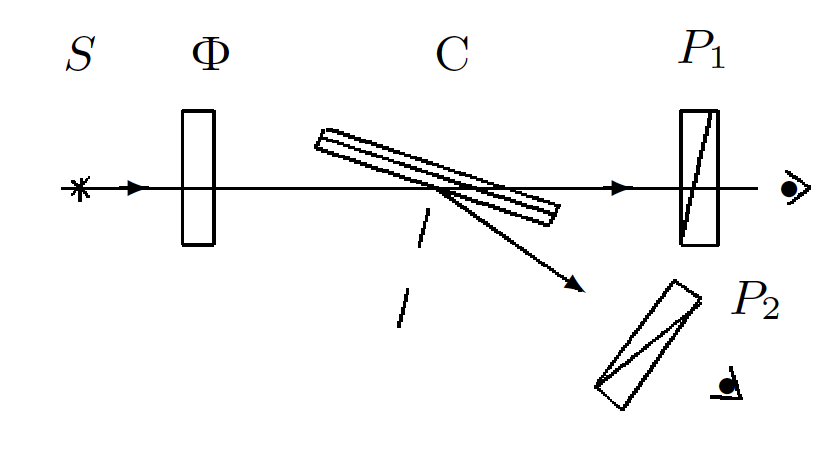
\includegraphics[width=0.3\linewidth]{6}
	\caption{Исследование стопы}
	\label{ris 6}
\end{figure}

Осветим стопу неполяризованным светом и, рассматривая через поляроиды $P_1$ и $P_2$ (рис. \ref{ris 6}) отражённый от стопы и преломлённый лучи, определим в них ориентацию вектора $ \vec{E} $. Наблюдая прошедший через стопу стеклянных пластинок луч света, убеждаемся в том, что плоскости поляризации у отражённого и преломлённого лучей взаимно перпендикулярны.

\subsection*{Двоякопреломляющие пластины}

\begin{figure}[h] 
	\centering
	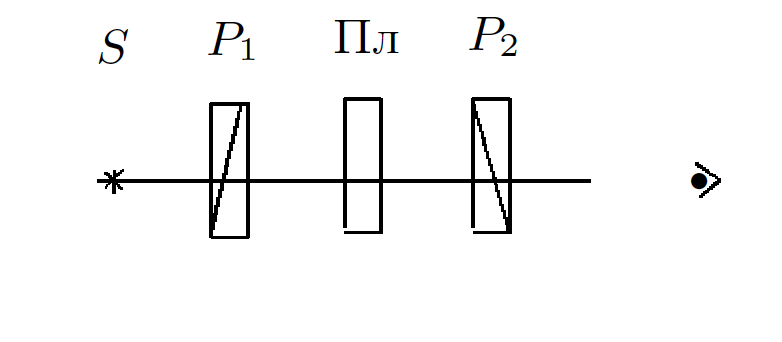
\includegraphics[width=0.3\linewidth]{7}
	\caption{Определение главных направлений в пластинках}
	\label{ris 7}
\end{figure}

Определим главные направления двоякопреломляющих пластин. 

Поставим кристаллическую пластинку между скрещенными поляроидами (рис. \ref{ris 7}). Вращая пластинку вокруг направления луча и наблюдая за интенсивностью света, проходящего сквозь второй поляроид, определим, при каком условии главные направления пластинки совпадают с разрешёнными направлениями поляроидов.

Итого получим:

\vspace{1mm}
\begin{center}
\begin{tabular}{|c|c|c|}
	\hline
	№ пластинки & минимальная интенсивность & максимальная интенсивность \\
	\hline
	1 & $96^\circ$ & $66^\circ$ \\
	\hline
	2 & $48^\circ$ & $22^\circ$ \\
	\hline
\end{tabular}
\end{center}


\subsection*{Пластинки $ \lambda/2, \lambda/4 $}

Для выделения пластин $ \lambda/2, \lambda/4 $ Добавим к схеме, изображённой на рис. \ref{ris 7}, зелёный фильтр и установим разрешённое направление поляризатора горизонтально, а главные направления исследуемой пластинки~---~под углом $ 45^\circ $ к горизонтали.

Пластинка в четверть длины волны создаёт сдвиг фаз на $\pi/2$, тем самым обеспечивая круговую поляризацию. На опыте это можно наблюдать следующим образом: если при вращении анализатора интенсивность света не меняется, то мы наблюдаем круговую поляризацию. В нашем эксперименте такие свойства проявляются у пластинки 2.

В случае с пластинкой в половину длины волны происходит только поворот плоскости колебаний вектора напряжённости электрического поля с переходом в другой квадрант, тип поляризации при этом не изменяется. Таким образом, свет остаётся линейно поляризованным, и при вращении анализатора интенсивность света изменяется. В нашем эксперименте такие свойства проявляются у пластинки 1.

\subsection*{Быстрая и медленная оси $ \lambda/4 $}

Определим "<быструю"> и "<медленную"> оси в пластинке $ \lambda/4 $.

Поставим между скрещенными поляроидами пластинку чувствительного оттенка, имеющую вид стрелки, и убедимся, что эта пластинка не меняет поляризацию зелёного света. Уберем зелёный фильтр и убедимся, что стрелка имеет пурпурный
цвет. Это объясняется тем, что зелёная компонента линейно поляризованного света при прохождении пластинки не меняет поляризации и задерживается вторым поляроидом.

\begin{figure}[h] 
	\centering
	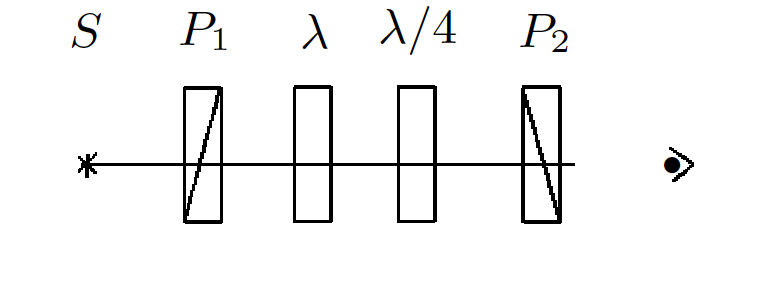
\includegraphics[width=0.3\linewidth]{8}
	\caption{Определение направлений большей и меньшей скорости}
	\label{ris 8}
\end{figure}

Добавим к схеме пластинку $ \lambda/4 $
(рис. \ref{ris 8}), главные направления которой совпадают с главными направлениями пластины $ \lambda $ и ориентированы
под углом $ 45^\circ $ к разрешённым направлениям скрещенных поляроидов.
При повороте рейтера со стрелкой на $ 180^\circ $ вокруг вертикальной оси
цвет стрелки меняется от зелёно-голубого до оранжево-жёлтого. В первом случае у нас "<быстрая"> ось (они совпадают), во втором~---~медленная, согласно теории из пункта <<Пластинка чувствительного света>>.

\subsection*{Интерференция поляризованных лучей}

Устанавливаем направление "<быстрой"> оси пластины $ \lambda/4 $ горизонтально.

Исследуем интерференцию поляризованных лучей. Для этого расположим между скрещенными поляроидами мозаичную слюдяную пластинку. Она собрана из 4-х узких полосок слюды, лежащих по сторонам квадрата (две полоски "<толщиной"> $ \lambda/4 $ и по одной~---~$ \lambda/2 $ и $ 3\lambda/4 $). В центральном квадратике слюды нет. Главные направления всех пластинок ориентированы параллельно сторонам квадрата.

Вращая пластинку, пронаблюдаем за изменениями в отдельном квадратике. У нас изменяется интенсивность с периодичностью $\pi/4$. Это происходит в силу того, что в этом случае меняется поляризация. 

Не трогая пластинки, повращаем второй поляроид. Теперь при неизменной интенсивности, изменяется цвет с той же периодичностью $\pi/4$. В данном случае это объясняется тем, что меняется сдвиг фаз.

\section*{Вывод}

Таким образом, мы ознакомились с методами получения и анализа поляризованного света. Измерили коэффициент преломления эбонита. Также мы поняли, что свойства поляризованного света можно применять для исследования оптических характеристик различных приборов и веществ.

\end{document}